\section{Evaluation und Diskussion}

\subsection{Testumgebung}

Um zu testen ob die Implementierung die Anforderungen erfüllen kann, mussten Test-bilder geschossen werden.

So dass die Test-Bilder genau sind und aus den resultierenden Posenschätzungen die Genauigkeit bestummen werden kann, wurde eine Testumgebung aufgebaut.

\begin{figure}[H]
    \centering
    \begin{subfigure}[h]{0.5\textwidth}
        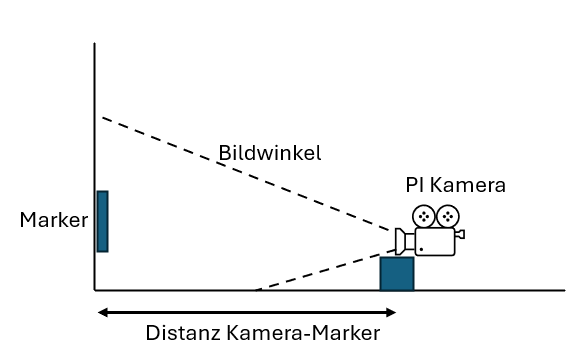
\includegraphics[width=0.5\textwidth]{graphics/Skizze_TestUmgebung.PNG}\hfill%
        \caption{Skizze der Testumgebung}
        \label{fig:SkizzeTestumgebung}
    \end{subfigure}
    \quad
    \begin{subfigure}[h]{0.5\textwidth}
        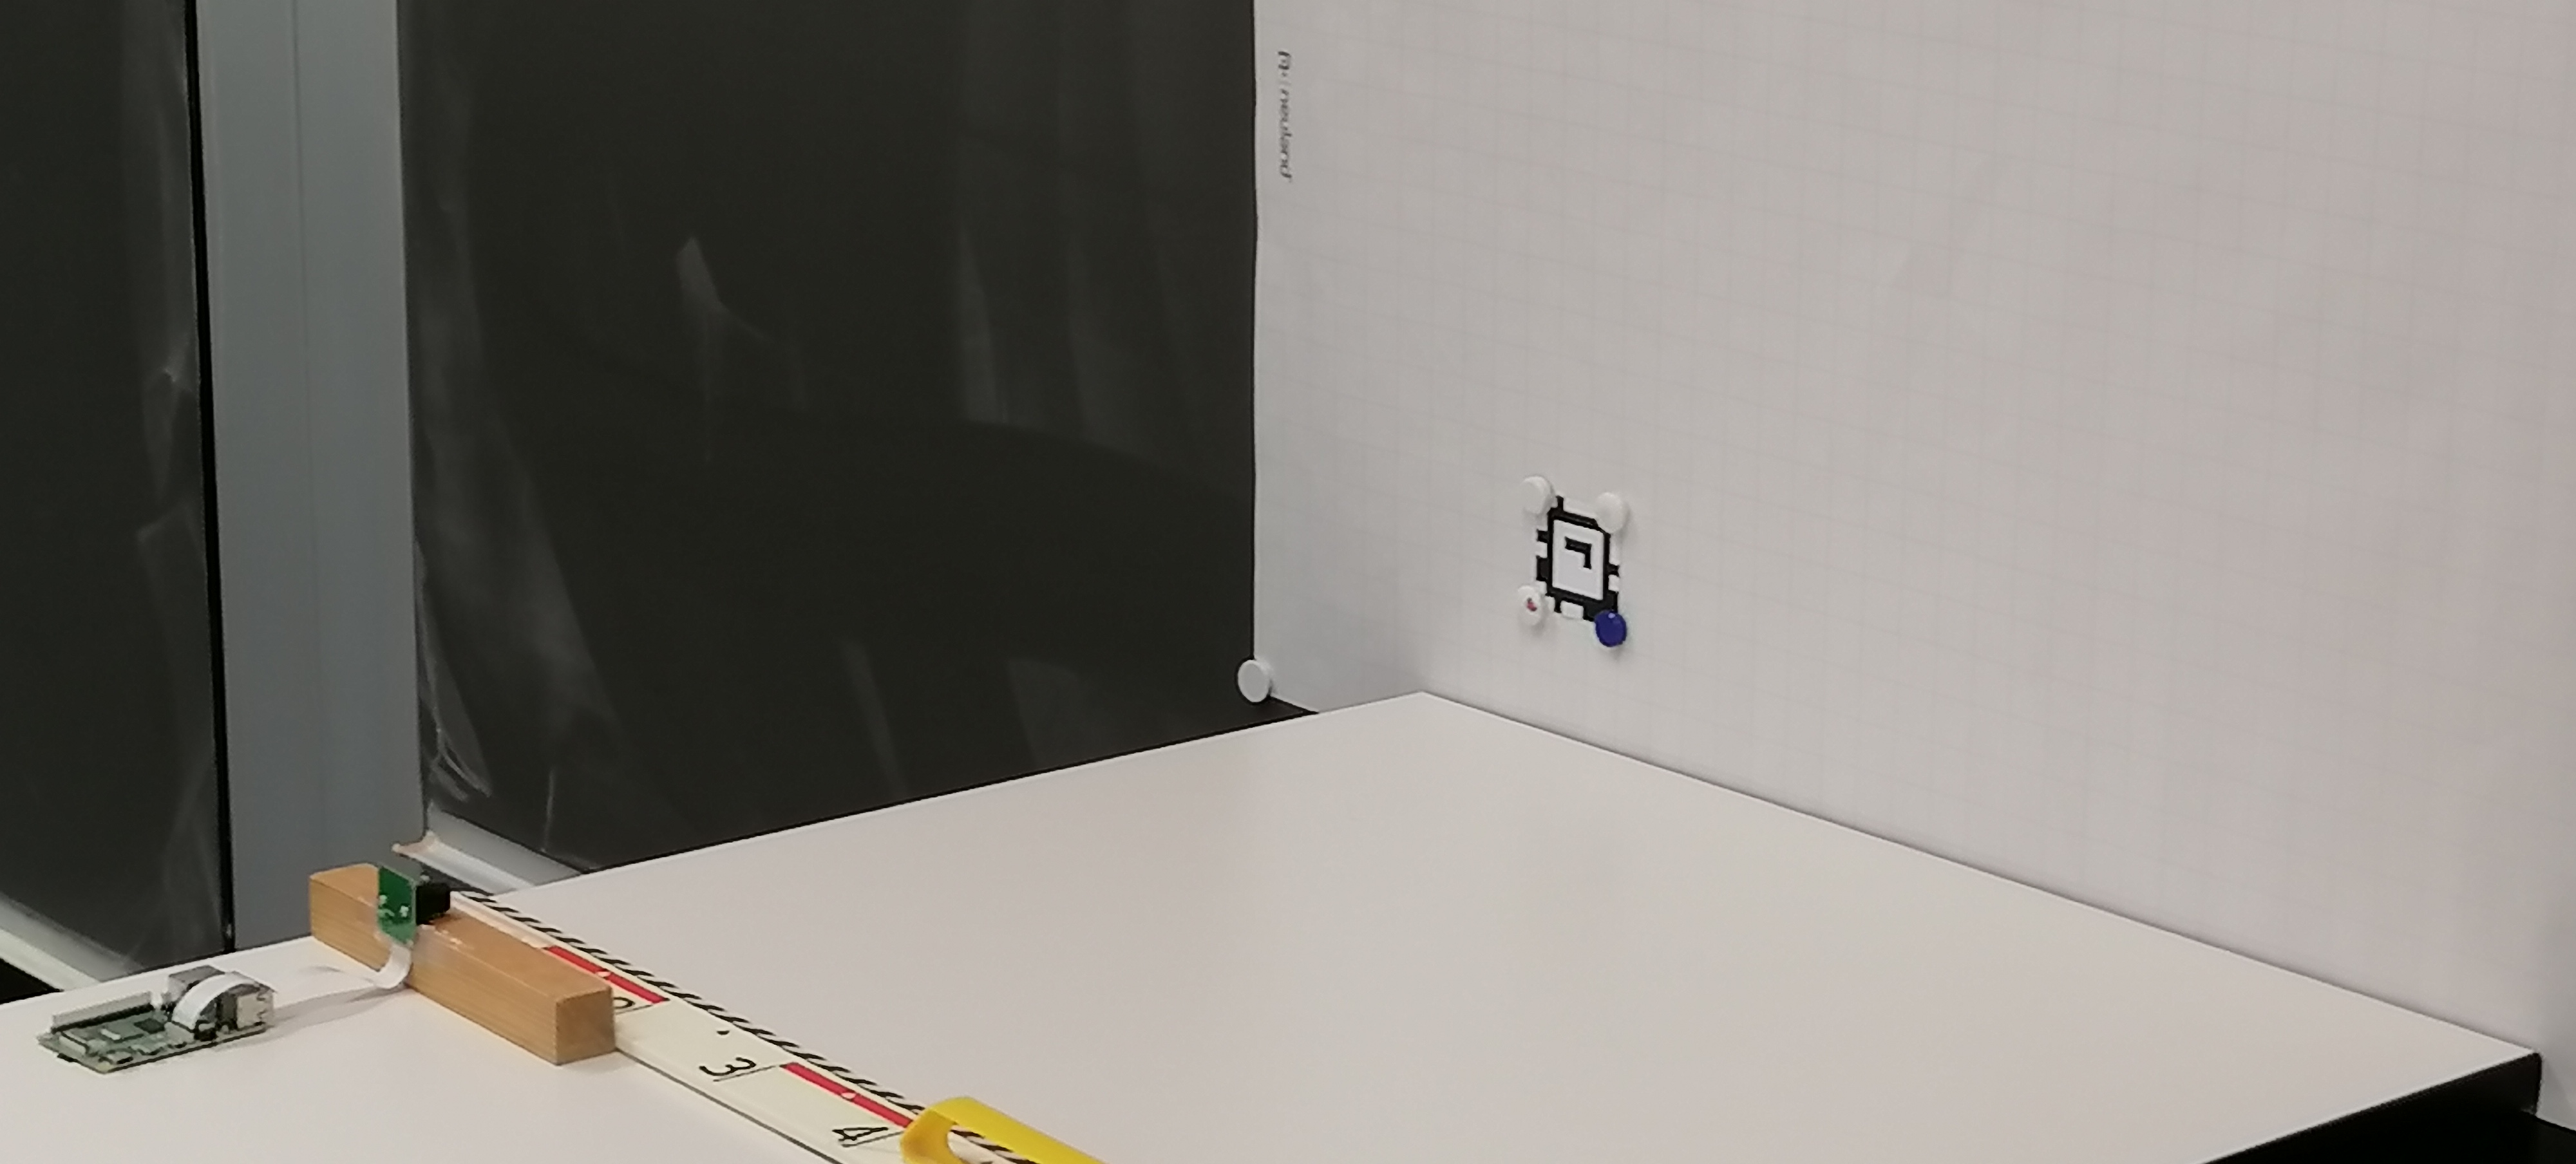
\includegraphics[width=0.5\textwidth]{graphics/TestUmgebung.jpg}\hfill%
        \caption{Implementierung der Testumgebung}
        \label{fig:Testumgebung}
    \end{subfigure}
    \caption{Beschreibung der Testumgebung}
\end{figure}

Die Abbildung \ref{fig:SkizzeTestumgebung} beschreibt wie die Testumgebung aufgebaut werden sollte.
Die Kamera sollte auf einem Objekt stabilisiert werden, um ein stabileres Bild zu bekommen und dass die Kamera höher gelagert ist und so mehr sehen kann.

Die Marker sollten auf einer Wand befestigt werden. 
Um einen fairen Vergleich zwischen Apriltag und ArUco machen zu können, wurden beide für die Posenschätzung nebeneinander auf einem Bild Fotografiert.
Dies stellt sicher dass beide Marker gleich entfernt sind und kleine Verschiebungen beide beinträchtigen.

Die Test-Fotos wurden von den Distanzen 75 cm, 100 cm, 150 cm und 200cm.
75 cm und 200 cm sind jeweils die Mindesthöhe und die Maximalhöhe, bei welcher das System funktionieren sollte.
100 cm und 150 cm wurden gewählt, um sehen wie die Ungenauigkeit sich über die Distanzen entwickelt.

Bei der Abbildung \ref{fig:Testumgebung} wird gezeigt wie die Implementierung der Skizze aussieht. 
Es wurde die Raspberry Pi Kamera Model B Rev 2.0 als Test-Kamera benutzt, welche auf einen Holzblock stabilisiert wurde.
Mit einem 1 Meter Lineal wurde sichergestellt, dass der Holzblock und damit die Kamera relativ zu den Marker gerade war.
Mit einem Messgerät wurde die Distanz vom Marker zur Kamera gemessen. 
Dabei musste noch die Länge des Objektives mitberechnet werden, da das Bild vom Sensor gemacht wird und von dort die Posenschätzung durchgeführt wird.

\subsection{Posenschätzung Marker}

Um die Anforderungen zu erfüllen, darf die Posenschätzung der Marker auf der X- und Y-Koordinate eine Ungenauigkeit von maximal 2cm besitzen. 
Auf der Z-Koordinate darf es maximal 1cm Ungenauigkeit besitzen.

\begin{table}[!htb]
    \caption{Resultate: X-Translation}
    \label{tab:xTrans}
    \begin{subtable}{.5\linewidth}
        \caption{Apriltags}
        \label{tab:xTransApril}
        \begin{tabular}{|l|l|l|l|l|c|}
            \hline
            Erwartet / Distanzen & 75cm & 100 cm & 150 cm & 200 cm  & Mittlere Abweichung\\
            \hline
            Erwartet: -8 cm &          & -7.54 cm & -7.30 cm & -7.80 cm & 0.45 cm\\
            \hline
            Erwartet: -6 cm &          & -6.01 cm & -5.83 cm  & -5.86 cm & 0.11 cm\\
            \hline
            Erwartet: -4 cm & -3.70 cm & -4.03 cm & -3.98 cm & -3.68 cm & 0.17 cm\\
            \hline
            Erwartet: -2 cm & -1.82 cm & -2.05 cm & -1.99 cm & -1.95 cm & 0.07 cm\\
            \hline
            Erwartet: 2 cm  & 2.29 cm & 1.71 cm & 1.55 cm & 1.80 cm & 0.31 cm\\
            \hline
            Erwartet: 4 cm  & 4.38 cm & 3.35 cm  & 3.50 cm & 3.50 cm & 0.51 cm\\
            \hline
        \end{tabular}
    \end{subtable}
    \\[\smallskipamount]
    \begin{subtable}{.5\linewidth}
        \caption{ArUco}
        \label{tab:xTransAruco}
        \begin{tabular}{|l|l|l|l|l|c|}
            \hline
            Erwartet / Distanzen & 75 cm & 100cm & 150cm & 200cm & Mittlere Abweichung\\
            \hline
            Erwartet:   -8 cm &          & -7.69 cm & -7.53 cm  & -8.05 cm & 0.28 cm\\
            \hline
            Erwartet:   -6 cm &          & -6.05 cm & -6.06 cm & -6.03 cm & 0.05 cm \\
            \hline
            Erwartet:   -4 cm & -3.91 cm & -4.06 cm & -4.13 cm & -3.76 cm & 0.13 cm \\
            \hline
            Erwartet:   -2 cm & -1.80 cm & -2.10 cm & -2.13 cm & -2.01 cm &  0.11 cm\\
            \hline
            Erwartet:   2 cm  & 2.09 cm & 1.76 cm & 1.56 cm & 1.71 cm & 0.26 cm\\
            \hline
            Erwartet:   4 cm  & 4.20 cm & 3.35 cm & 3.45 cm & 3.49 cm & 0.48 cm \\
            \hline
        \end{tabular}
    \end{subtable} 
\end{table}

Die Tabelle \ref{tab:xTrans} zeigt die Resultate von den X-Translationen. 
Wie an der Tabelle \ref{tab:xTransApril} und \ref{tab:xTransAruco} zu sehen ist, erfüllen beide die Anforderung von maximal 2 cm Ungenauigkeit.
Bei \ref{tab:xTransApril} hat eine Durchschnittliche mittlere Abweichung von 0.27 cm. 
Bei \ref{tab:xTransAruco} hat eine Durchschnittliche mittlere Abweichung von 0.22 cm. 

\begin{table}[!htb]
    \caption{Resultate: Y-Translation}
    \label{tab:yTrans}
    \begin{subtable}{.5\linewidth}
        \caption{Apriltags}
        \label{tab:yTransApriltag}
        \begin{tabular}{|l|l|l|l|l|c|}
            \hline
            Erwartet / Distanzen & 75 cm & 100 cm & 150 cm & 200 cm & Mittlere Abweichung\\
            \hline
            Erwartet:   -8 cm &          & -8.54 cm & -9.61 cm & -9.91 cm & 1.35 cm\\
            \hline
            Erwartet:   -6 cm & -6.55 cm & -6.44 cm  & -7.29 cm & -7.70 cm & 1.00 cm\\
            \hline
            Erwartet:   -4 cm & -4.76 cm & -4.38 cm & -5.32 cm & -5.77 cm & 1.06 cm\\
            \hline
            Erwartet:   -2 cm & -2.36 cm  & -2.29 cm & -3.00 cm & -3.37 cm & 0.75 cm\\
            \hline
        \end{tabular}
    \end{subtable}
    \\[\smallskipamount]
    \begin{subtable}{.5\linewidth}
        \caption{ArUco}
        \label{tab:yTransAruco}
            \begin{tabular}{|l|l|l|l|l|c|}
            \hline
            Erwartet / Distanzen & 75 cm & 100 cm & 150 cm & 200 cm & Mittlere Abweichung \\
            \hline
            Erwartet:   -8 cm &          & -8.30 cm & -9.10 cm & -9.93 cm & 1.11 cm \\
            \hline
            Erwartet:   -6 cm & -6.27 cm  & -6.07 cm & -7.10 cm & -7.73 cm & 0.79 cm\\
            \hline
            Erwartet:   -4 cm & -4.44 cm & -4.25 cm & -5.07 cm & -6.04 cm & 0.95 cm \\
            \hline
            Erwartet:   -2 cm & -2.21 cm & -2.10 cm  & -2.83 cm & -3.81 cm & 1.26 cm\\
            \hline
        \end{tabular}
    \end{subtable} 
\end{table}

Die Tabelle \ref{tab:yTrans} zeigt die Resultate von den X-Translationen. 
Wie an der Tabelle \ref{tab:yTransApriltag} und \ref{tab:yTransApriltag} zu sehen ist, erfüllen fast beide die Anforderung von maximal 2 cm Ungenauigkeit.
Bei \ref{tab:yTransApriltag} hat eine Durchschnittliche mittlere Abweichung von 1.04 cm. 
Bei \ref{tab:yTransAruco} hat eine Durchschnittliche mittlere Abweichung von 1.03 cm.

Bei 200cm Abstand hat ArUco eine grössere Ungenauigkeit als Apriltag. 
In der Y-Translation von -4 cm überschreitet ArUco Marker die Ungenauigkeit von maximal 2 cm mit 2.04 cm. 

\begin{table}[!htb]
    \caption{Resultate: Z-Translation}
    \label{tab:zTrans}
    \begin{subtable}{.5\linewidth}
        \caption{Apriltags}
        \label{tab:zTransApril}
        \begin{tabular}{|l|l|l|l|l|c|}
            \hline
            Distanzen & 75 cm & 100 cm & 150 cm & 200 cm &  Mittlere Abweichung\\
            \hline
            &75.72438 & 99.95 cm & 150.05 cm & 200.00 cm & 0.21 cm\\
            \hline
        \end{tabular}
    \end{subtable}
    \\[\smallskipamount]
    \begin{subtable}{.5\linewidth}
        \caption{ArUco}
        \label{tab:zTransAruco}
        \begin{tabular}{|l|l|l|l|l|c|}
            \hline
            Distanzen & 75 cm & 100 cm & 150 cm & 200 cm  &  Mittlere Abweichung \\
            \hline
            & 76.49 cm & 101.66 cm & 152.58 cm & 203.49 cm & 2.30 cm\\
            \hline
        \end{tabular}
    \end{subtable} 
\end{table}

Diese Tabelle\ref{tab:zTrans} zeigt die Genauigkeiten von der Z-Translation.
Bei \ref{tab:zTransApril} hat eine Durchschnittliche mittlere Abweichung von 0.23 cm. 
Bei \ref{tab:zTransAruco} hat eine Durchschnittliche mittlere Abweichung von 2.3 cm.

In der Z-Translation, überschreitet der ArUco Marker die maximale Ungenauigkeit bei allen Distanzen.
Die Apriltags erfüllt die Anforderungen bei allen Distanzen.


\begin{table}[!htb]
    \caption{Resultate: Z-Rotation}
    \label{tab:zRot}
    \begin{subtable}{.5\linewidth}
        \caption{Apriltags}
        \label{tab:zRotApril}
        \begin{tabular}{|l|l|l|l|l|c|}
            \hline
            Erwartet / Distanzen & 75 cm & 100 cm & 150 cm & 200 cm & Mittlere Abweichung\\
            \hline
            Erwartet:   -60\degree & -59.97\degree & -59.89\degree & -59.75\degree   & -59.74\degree & 0.16\degree\\
            \hline
            Erwartet:   -45\degree & -44.08\degree & -44.04\degree & -43.97\degree & -43.97\degree & 0.99\degree\\
            \hline
            Erwartet:   -30\degree & -31.33\degree  & -31.43\degree & -31.33\degree & -31.61\degree & 1.42\degree\\
            \hline
            Erwartet:   30\degree  & 32.57\degree & 32.54\degree  & 32.19\degree & 32.32\degree & 2.41\degree\\
            \hline
            Erwartet:   45\degree  & 45.44\degree & 45.46\degree & 45.50\degree & 45.62\degree & 0.51\degree\\
            \hline
            Erwartet:   60\degree  & 61.39\degree & 60.52\degree & 60.58\degree & 60.79\degree & 0.82\degree\\
            \hline
        \end{tabular}
    \end{subtable}
    \\[\smallskipamount]
    \begin{subtable}{.5\linewidth}
        \caption{ArUco}
        \label{tab:zRotAruco}
        \begin{tabular}{|l|l|l|l|l|c|}
            \hline
            Erwartet / Distanzen & 75 cm & 100 cm & 150 cm & 200 cm & Mittlere Abweichung \\
            \hline
            Erwartet:   -60\degree & -58.92\degree & -59.00\degree & -59.20\degree & -59.11\degree & 0.94\degree\\
            Erwartet:   -45\degree & -44.50\degree & -43.99\degree & -44.78\degree & -43.42\degree & 0.83\degree\\
            Erwartet:   -30\degree & -30.23\degree  & -29.98\degree & -29.86\degree  & -29.77\degree & 0.15\degree\\
            Erwartet:   30\degree  & 31.71\degree & 31.66\degree & 32.03\degree & 31.76\degree & 1.79\degree\\
            Erwartet:   45\degree  & 45.84\degree & 45.93\degree & 46.52\degree & 45.90\degree & 1.05\degree\\
            Erwartet:   60\degree  & 61.69\degree & 61.60\degree & 61.79\degree & 61.15\degree & 1.56\degree\\
            \hline
        \end{tabular}
    \end{subtable} 
\end{table}

Um die Anforderungen zu erfüllen, muss die Z-Rotatation eine maximale Ungenauigkeit von 2\degree besitzen.
Bei der Tabelle \ref{tab:zRotApril} ist zu sehen, dass nur bei 30\degree diese maximale Ungenauigkeit überschritten wurde.
Bei der Tabelle \ref{tab:zRotAruco} ist zu sehen, dass auch nur bei 30\degree diese maximale Ungenauigkeit überschritten wurde, aber nur bei 150cm.
Bei \ref{tab:zRotApril} hat eine Durchschnittliche mittlere Abweichung von 1.05\degree. 
Bei \ref{tab:zTransAruco} hat eine Durchschnittliche mittlere Abweichung von 1.05\degree.



\subsection{Mittelpunkt-Berechnung}

\subsection{Diskussion}